\documentclass[10pt,twocolumn]{article}

% use the oxycomps style file
\usepackage{oxycomps}

% usage: \fixme[comments describing issue]{text to be fixed}
% define \fixme as not doing anything special
\newcommand{\fixme}[2][]{#2}
% overwrite it so it shows up as red
\renewcommand{\fixme}[2][]{\textcolor{red}{#2}}
% overwrite it again so related text shows as footnotes
%\renewcommand{\fixme}[2][]{\textcolor{red}{#2\footnote{#1}}}

% read references.bib for the bibtex data
\bibliography{references}

% include metadata in the generated pdf file
\pdfinfo{
    /Title (An Analysis on the Tesseract Library for Text Recognition and Extraction)
    /Author (Luis Martinez)
}

% set the title and author information
\title{An Analysis on the Tesseract Library for Text Recognition and Extraction}
\author{Luis Martinez}
\affiliation{Occidental College}
\email{lmartinez3@oxy.edu}

\begin{document}

\maketitle

\section{Problem Statement}

	As industries increasingly move towards digitization, the ability to extract text from images and other visual formats has become crucial for efficient data processing and analysis. Optical Character Recognition (OCR) is the key process enabling this functionality by allowing text to be identified and converted into machine-readable formats. Moving forward, this paper will use the term OCR to refer to this process to be succinct. Commercial OCR tools like Google Cloud Vision API and Amazon Textract exist to address the growing need for OCR tools, however their effectiveness often comes at a significant financial cost. These expenses can pose barriers for emerging businesses and non-commercial users, such as students and researchers. Tesseract OCR, an open-source programming library, offers a cost-effective alternative and has benefited from decades long development.\paragraph{} However, Tesseract often struggles under suboptimal conditions - such as poor lighting, imperfect document scans, and digital artifacts - sometimes failing to even recognize the presence of text entirely. This paper seeks to address these limitations by systematically investigating how various text and image characteristics impact Tesseract's OCR accuracy, identifying factors contributing to its performance variability, and proposing evidence-based recommendations to enhance its reliability. Ultimately, these findings aim to contribute to the broader accessibility and usability of OCR technology, especially for underfunded and independent users. 

\section{Technical Background}

To understand the limitations of Tesseract explored in this paper, it is essential to delve into how it operates and some of the math that underlines its functionality. As mentioned above, Tesseract is an open-source OCR engine that attempts to extract text from images. It was initially developed by Hewlett-Packard Laboratories until 2005 when HP open-sourced it. Then Google further developed it between 2006 and 2018\cite{github_repo}. Tesseract works via a multistage pipeline consisting of the following steps: preprocessing, layout analysis, character recognition, and adaptive learning\cite{Overview_Akhil} \cite{Overview_Smith}. 

\subsection{Adaptive Thresholding}

The first step in Tesseract’s pipeline is adaptive thresholding, which transforms a grayscale image into a black-and-white image. This step ensures that the text in the image stands out against the background. To determine what parts of the image become background / background, Tesseract uses the Otsu method, a mathematical technique that determines the optimal threshold for deciding what the final color of a pixel will be. To achieve this, Otsu’s method determines the intensity of each pixel on a scale of 0 (black) to 255 (white). Then, calculates a threshold t by evaluating all possible thresholds and selecting the one that minimizes the "variance" (a measure of spread) within each group using the formula following formula: \cite{Overview_Akhil}.
\[
\sigma^2_{\omega}(t) = \omega_0(t)\sigma_0^2(t) + \omega_1(t)\sigma_1^2(t)
\]

Here, $\omega_0$ and $\omega_1$ are probabilities of pixel classes, and $\sigma_0^2$, $\sigma_1^2$ are their variances\cite{Overview_Akhil}.
If the image has varying lighting, Tesseract applies this technique to small sections rather than the entire image to try to improve accuracy. This technique is called local adaptive threshold.




\subsection{Page Layout Analysis}

The next step in the pipeline is layout analysis, where Tesseract attempts to divide the image into regions of text and non-text (i.e., images, diagrams, whitespace, etc.). Tesseract does this in three steps, ideally saving time by focusing only on areas likely to have text.

\begin{enumerate}
    \item \textbf{Connected Component Analysis:} Tesseract attempts to identify clusters of connected black pixels called \textit{Blobs}. Given that there is no noise or artifacts in the image, these blobs will represent individual letters and punctuation. It also helps filter out non-text, as blobs that are overly large relative to the median blob size of the region are ignored.
    
    \item \textbf{Tab-Stop Detection:} Using the \textit{Leptonica} (an image processing library), Tesseract tries to detect vertical and horizontal lines to identify the boundaries between columns of text and to separate multi-column text.
    
    \item \textbf{Row and Line Detection:} In this step, Tesseract groups the blobs into rows of text by checking their proximity to each other and whether they overlap vertically. If an image is skewed, it uses a least median of squares fitting method to estimate a straight baseline for each row. This works by calculating the potential baseline that minimizes the squared difference between the points/pixels.
    
    \item \textbf{Baseline Fitting:} To further refine the baselines for each row, Tesseract uses a quadratic spline, a smooth curve calculated by minimizing the errors between the predicted and actual positions of blobs \cite{geeks}. This further helps Tesseract identify text on slightly curved lines, such as those seen in poorly scanned book pages \cite{Overview_Smith} \cite{Overview_Akhil}.

    
\end{enumerate}

\subsection{Character Segmentation and Recognition}
After attempting to identify the rows and columns of the image, Tesseract tries to break text into words and then into characters. To achieve this, it uses one of two methods depending if the text is Fixed-Pitch (consistently spaced characters) if it is Proportional Text (inconsistently spaced characters).
\begin{enumerate}
    \item \textbf{Fixed-Pitch Text:} For consistently space characters Tesseract, attempts to detect the uniform spacing in order to directly chop the text in character-sized segments using the fixed pitch as a guide \cite{Overview_Smith}\cite{Overview_Akhil}.

    \item \textbf{Proportional Text:} For inconsistently spaced characters, it attempts to measure the gaps between the blobs within a given baseline. After this it classifieds spaces into either “definite” (clear separation) or “fuzzy” (unclear spacing). Tesseract later attempts to make final determination on the fuzzy spaces during word recognition\cite{Overview_Smith}\cite{Overview_Akhil}.
    
\end{enumerate}

\subsection{Word Recognition}
Once Tesseract has made its attempt to segment the words into characters, it begins the recognition process which occurs in two pass to improve accuracy.

\begin{enumerate}
    \item \textbf{Static Classifier:} In this first pass, Tesseract tries to classify each blob by comparing its features to those of the pre-trained prototypes in the static classifier. The researchers developed these prototypical features by clustering the 4-dimensional feature vectors (x-position, y-position, direction, and length) for each of a character’s polygonal outline \cite{Overview_Akhil}. This use of multidimensional feature vectors is the source of Tesseract’s name.
    \paragraph{}To measure how close the detected features are to the prototypical features, Tesseract uses a distance metric. It calculates the distance between each feature as:
    \[
d_f = d^2 + w\theta^2
\]

\begin{itemize}
    \item $d$: Euclidean distance between a feature and prototype.
    \item $\theta$: Angular difference (orientation of the feature).
    \item $w$: Weight factor adjusting the influence of angle differences.
\end{itemize}
After this calculation, the classifier ranks the possible matches and selects the character with the highest confidence score. In situations where multiple characters incorrectly combined into a single blob, Tesseract attempts to identify potential “chop points” based on the concavity of vertices in the character outline. It then iteratively tests the chop points to find which has the best segmentation \cite{Overview_Smith}\cite{Overview_Akhil}.
\paragraph{}

    \item \textbf{Adaptive Classification:} During this second pass, Tesseract takes the recognized characters from the first pass and attempts to use them to train an adaptive classifier that dynamically adjusts to the specific font or style used in the image. If Tesseract was not confident in its recognition of characters during the first pass, it will use this new adaptive classifier to try to improve its results \cite{Overview_Smith}\cite{Overview_Akhil}.
\end{enumerate}


\subsection{Linguistic Analysis}
During the recognition phase, Tesseract attempts to utilize a lightweight linguistic analysis to improve the accuracy of its output. During character recognition, it generates multiple guesses for each word based on the different segmentations and classifier outputs. It then ranks each guess based on the following categories: “Top frequent word, Top dictionary word, Top numeric word, Top UPPERcase word, Top lower case word (with optional initial upper), Top classifier choice word” \cite{Overview_Smith}. Tesseract then selects the guess with the highest combined output. Ideally, this process ensures Tesseract corrects  common errors, like mistaking the letter “o” with zero. After character recognition, Tesseract relies on the classifier confidence scores to determine the most likely sequence of characters. This allows it to handle non-standard words such as names, technical terms or foreign languages, although with a reduced accuracy \cite{Overview_Smith}.
\newline \newline
Overall, Tesseract is a powerful OCR engine that combines adaptive thresholding, baseline fitting, and dual-pass classification to try to handle diverse text styles effectively. While its adaptive learning enhances recognition accuracy within documents, it struggles with noisy or distorted inputs, relying heavily on clean, high-quality images. Its simplistic linguistic analysis and static training also limit its ability to handle ambiguous or highly stylized text. These challenges underscore the need for enhancements in processing suboptimal inputs and improving contextual understanding, which this paper aims to address.

\section{Prior Work}
Existing research on Tesseract predominantly emphasizes its use within larger projects rather than examining the tool itself. As a result of this, there is limited exploration of the parameters influencing its accuracy, but numerous studies explore methods to preprocess images for a given purpose. There are also notable papers that, while not experimenting with the accuracy-affecting vectors of Tesseract, offer valuable insights into its functionality.

\subsection{Tesseract Insights}
The two papers that significantly aided my understanding of Tesseract’s design and functionality are Smith’s \textit{An overview of the Tesseract OCR Engine}\cite{Overview_Smith} and Akhil’s \textit{An overview of Tesseract OCR Engine}\cite{Overview_Akhil}. Smith’s 2007 paper provides a historical and architectural perspective on Tesseract, detailing its evolution from an HP Labs research project to an open-source OCR tool. Furthermore, it outlines the core components of Tesseract’s processing pipeline and the ways in which it differs from earlier and  alternative OCR tools. While informative, Smith’s paper only provides a high-level overview of Tesseract, lacking information on the mathematical principles that underpin Tesseract’s functionality (Smith). Akhil’s 2016 paper complements Smith’s overview by delving into the mathematical equations used for baseline determination and character recognition via four feature vectors. However, it lacks coverage of the linguistic analysis performed by Tesseract. Despite these individual limitations, the combination of insights from both papers provided me with a comprehensive understanding of Tesseract’s inner workings, especially the knowledge of the four feature vectors which heavily influence the parameters I chose to use. 


\subsection{Preprocessing Steps in OCR Papers}
Each of the studies I have reviewed explored preprocessing steps to varying degrees to enhance Tesseract’s accuracy. These steps are essential as they improve the image clarity and highlight features directly impact the recognition systems of the OCR. For example, in The Use of OCR Number Recognition for Food Tracking and Tracing, the researchers struggled with removing horizontal lines from the labels they had photographed as shown in Figure~\ref{fig:food}\cite{food}.

\begin{figure}[h!]
    \centering
    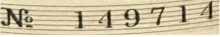
\includegraphics[width=\linewidth]{Figures/food_fig.png}
    \caption{Example Food Label.}
    \label{fig:food}
\end{figure}

Although the paper does not explicitly explain this, the horizontal lines likely disrupted the row and column detection process and interfered with character segmentation, potentially leading Tesseract to interpret the text as a single large blob. To address this issue, the researchers applied image dilation (increases of white space\cite{cv_dilate}) and gaussian blur (the application of a gaussian function to smooth/blur an image to assist in noise reduction\cite{cv_dilate} \cite{medium_gauss}). After this, they applied Otu’s method and erosion (reduction of white space\cite{cv_dilate}). Crucially,  the researchers noted challenges with shadows but did not provide a solution, and they manually cropped their images\cite{food}. These details are important because they informed my creation of a control image and the decision to implement a method for assessing image lighting quality.
    
Another influential paper is \textit{An Automatic Number Plate Recognition System using OpenCV and Tesseract OCR Engine} which proposed an algorithm designed and optimized to extract the numbers from Ghanaian license plates. The OCR system begins by grayscaling the image. It then applies vertical and horizontal Sobel-Feldman convolution kernels to detect edges within the image\cite{automatic}. This step is crucial for locating rectangles that match the aspect ratio of standard license plates and enables the system to automatically identify and crop the potential license plate regions. Next, the system employs connected component analysis (“an algorithmic application of graph theory used to determine the connectivity of “blob”-like regions in a binary image”\cite{CCA}) to determine the best license plate candidate. Once it’s identified, the system separates and de-noises each character. For the last step of preprocessing, it reassembles the processed characters into a new image with the text drawn in a single line as illustrated in Figure~\ref{fig:plate} 2\cite{automatic}. 
\begin{figure}[h!]
    \centering
    
\includegraphics[width=\linewidth]{Figures/plate_fig.png}
    \caption{Processed Number Plate.}
    \label{fig:plate}
\end{figure}

The necessity of automatic cropping in this study combined with the manual cropping in the previously discussed paper reinforced my decision to create a control image rather than relying on a real-world image. This ensured that the accuracy of my tests would not be influenced by inconsistencies in the cropping process. Additionally, this step, combined with my prior experiments, highlighted the importance of determining adequate spacing between the image border and text to avoid overly aggressive cropping. Furthermore, their use of a single line of characters encouraged me to do the same in my testing since it showed that Tesseract could work under that condition, which would save processing time and digital storage space.

While the following papers did not influence this study as strongly as those previously discussed, they reinforced my choice of parameters to test and introduced novel ideas that, although not directly relevant to this work, could inform future research on Tesseract and other OCR systems. The first of these papers is  \textit{CV Content Recognition and Organization Framework based on YOLOv8 and Tesseract-OCR Deep Learning Models} which focuses on creating an improved system for extracting data from CVs. Beyond the preprocessing steps already mentioned, the researchers upscaled images to standard dimensions. However, the most notable difference in their process was the implementation of YOLOv8 (You Only Look Once) ,a real-time object detection algorithm, to generate bounding boxes for Tesseract\cite{yolo}. This approach enhanced OCR accuracy by functioning as an automated cropping mechanism, but decided not to incorporate it or similar tools due to it landing outside of the scope of my project. However, further analysis on Tesseract would benefit from testing with  object detection tools like YOLO should be used.  Another novel method appeared in the paper \textit{Detecting In-Game Toxicity via Bullet Hole Patterns Using Image Recognition}. As the title suggests, the study proposed detecting specific words generated by patterns of simulated bullet holes. The researcher used many of the same preprocessing methods that the other papers had used, but they added an image saturation step before the grayscaling in the attempt to amplify the contrast between the background and foreground elements\cite{bullets}. While this method was not applicable to my black-and-white control images, it warrants further exploration in studies using real-world images. I also reviewed other papers that largely reiterated common preprocessing techniques without offering significant novel implementations. The most notable of these, InkSight: Offline-to-Online Handwriting Conversion by Learning to Read and Write, was published in 2024 and  introduced innovative methods but fell outside the scope of this project\cite{inksight}.



\section{Methods}
This study consisted of two sets of testing designed to evaluate Tesseract's OCR accuracy under different conditions. In the first set of tests, the independent variable was the font type, while the dependent variable was Tesseract’s text recognition performance. The second set of tests used a calculated control image and tested a variety of parameters that I will explain in their relevant sections. 
\subsection{First Series of Testing}
Based on my understanding of Tesseract's operational mechanics, I selected a diverse set of fonts for testing. These included standard fonts such as Arial and handwritten-inspired fonts like Caveat. I also used Comic Sans and a special font called Opendyslexic which were believed to be better for people for dyslexia due to their spacing and shape design, and while this has been proven untrue by papers like \textit{The effect of a specialized dyslexia font, OpenDyslexic, on reading rate and accuracy}\cite{effects_of_dyslexia} and \textit{Do Dyslexia Fonts Actually Work?}\cite{do_dyslexia_fonts}, I thought they may have higher accuracy by making it easier for Tesseract to separate the characters and have similar letters be more distinct from one another. I sourced most of the fonts from Google Fonts\cite{googlefonts} and Free Fonts Family\cite{freefontsfamily}, and I directly sourced OpenDyslexic\cite{opendyslexic} from its official website. Ultimately, I gathered over 40 fonts including variations of those fonts such as bold and italicized styles.
To evaluate Tesseract's performance, I tested the following parameters: average line thickness, average angle between lines, average number of curves, and character spacing. I chose these metrics to explore how font characteristics impact Tesseract’s ability to recognize text:
\subsubsection{Parameter Calculation}
\begin{itemize}
\item \textbf{Average Line Thickness:} Using OpenCV, the script identified letter contours and measured the pixel thickness between these contours, averaging the values across all letters in the image.
\item \textbf{Average Angle Between Lines:} The script divided the contours into line segments and calculated the angle between adjacent segments.
\item \textbf{Average Number of Curves:} The script identified angular changes exceeding 15 degrees along the line segments, counting these as curves.
\item \textbf{Character Spacing:} Instead of analyzing spacing from rendered images, I directly extracted spacing data from font files using the FontTools library. This method ensured that font size did not introduce variability in the measurements. The outputed measurements were in EM units, a standard typographic measurement. 

\end{itemize}
For the test text, I chose Mary Shelley’s \textit{Frankenstein} semi-arbitrarily as I wanted to simulate a realistic use case. For image generation, I wrote a Python script using the Pillow image manipulation library and Matplotlib. Each test image measured 1000 x 800 pixels, with text rendered at a font size of 16. I chose font size 16 because, for most standard fonts, it approximates the spacing of college-ruled paper lines (0.71 cm) and aligns closely with the commonly used 12-point font for professional documents
By combining computational image analysis with font file metadata extraction, this methodology ensured consistency in evaluating the impact of font characteristics on Tesseract’s OCR performance.

\subsection{Second Series of Testing}
The second series of tests aimed to evaluate how specific parameters at varying intensities affected Tesseract’s ability to detect text. I used a control image as the baseline for these experiments. The control image featured the Arial font and the uppercase letter “A.” I selected Aerial for its high accuracy in the first testing series and its ubiquity in text applications. I chose the letter  “A” for simplicity and relevance, with the knowledge that any  future research should expand to randomized alphanumeric combinations. The image was 500 x 500 pixels and rendered in black and white to minimize extraneous variables and reduce computational demands.
\subsubsection{Control Image Design}
The control image incorporated parameters such as font size, number of characters, and character spacing (defined as the distance between adjacent letters, with a value of 1 representing one letter’s width). These parameters were chosen based on prior observations that Tesseract sometimes failed to detect text in images that were too small or sparsely populated. The images were generated using Matplotlib, with loops iterating over each parameter to systematically create test cases. The text detection frequency (whether Tesseract identified any text in the image) was recorded for each parameter configuration.
Following these analyses, the optimal control image parameters were determined to be:
\begin{itemize}
    \item Font Size: 20 (chosen for its high detection frequency and similarity to the height of college-ruled paper lines).
    \item Character Spacing: 1.
    \item Number of Characters: 4.
\end{itemize}
This control image is shown in Figure~\ref{fig:Control}
\begin{figure}[h!]
    \centering
    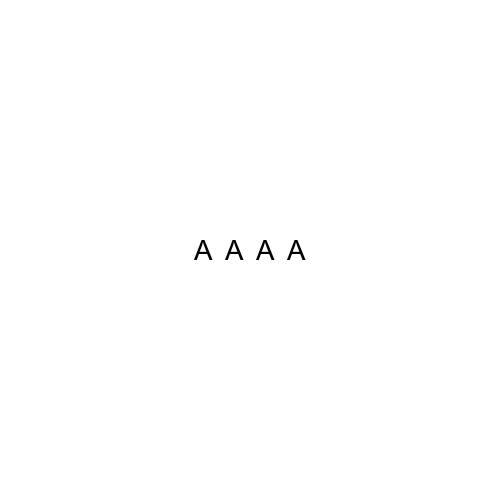
\includegraphics[width=\linewidth]{Figures/Control_Image.png}
    \caption{Control Image.}
    \label{fig:Control}
\end{figure}


\subsubsection{Tested Parameters}
After finalizing the control image, I tested the following parameters: slant, weight, white space, salt-and-pepper noise, and Perlin noise. I initially considered curviness as a parameter but excluded it due to challenges in implementing consistent and efficient modifications programmatically. I also considered use Parametric fonts like Roboto Flex but it proved impractical for this study due to their limited parameter ranges preventing extreme modifications to the font's appearance and development struggles due to its target usage being front-end development which I have very limted experience with.

\begin{enumerate}
    \item \textbf{Slant:}  Slant represents how far the text leans left or right, simulating skewed text in images. Initially, I tested slant values ranging from -30 to 30, but this range was later expanded to -60 to 60 to better highlight Tesseract’s limitations. It is important to note that these values are not in degrees, but will be converted to degrees later in the paper. To modify the slant value, the code took the coordinates of the text area, converted the values into a matrix,  and applied an affine transformation to those values. An affine transformation is a geometric transformation that preserves the proportions of lines without having to preserve the angles or lengths\cite{mathworld_affine}. This allowed me to change the slant while preserving the vertical height.\
    \item \textbf{Weight:}Weight is the relative thickness of the lines of the font.To adjust this parameter, I applied erosion and dilation transformations using the OpenCV library. While I considered an alternative approach involving manual vector manipulation or parametric fonts, it was ultimately impractical due to time constraints. Initial tests at a 20-point font size yielded unsatisfactory results, so I conducted additional experiments at a 50-point font size. The reasoning behind this adjustment is discussed in the Results and Discussion section.
    \item \textbf{White Space:} White space refers to the amount of empty space between the text and the edges of the image. I tested this parameter by programmatically creating variations of the control image with additional rows of white pixels added to the top and bottom of the image. The script then centered the text relative to the modified boundaries. This test was motivated by prior observations of Tesseract failing to detect text when there was insufficient border space. Future studies should explore the effects of white space in multi-line text scenarios, which were beyond the scope of this work due to time constraints.
    \item \textbf{Salt-and-Pepper Noise}: Salt-and-pepper noise introduces random black and white pixels into the image, simulating artifacts from poor scanning or image transfer. To apply this noise, I wrote a script that used a strength parameter ranging from 0 to 1, where the value represents the percentage of pixels affected. For example, a strength of 0.1 means 10 percent of the pixels were altered, evenly split between "salt" (white) and "pepper" (black) pixels. After an initial pass, I refined the testing by running the script with smaller increments to pinpoint the threshold where Tesseract could no longer detect text.
    \item \textbf{Perlin Noise:} Perlin noise introduces gradients of random noise to simulate uneven lighting conditions. Using the PerlinNoise Python library, I generated noise with varying intensity levels. The intensity parameter controlled the proportion of the image affected, with higher values creating darker and more pronounced gradients. This allowed me to assess how lighting inconsistencies impacted Tesseract’s accuracy.

\end{enumerate}
The methods employed in this study were designed to systematically evaluate Tesseract's performance under controlled conditions and across a range of realistic challenges. By testing key parameters such as slant, weight, spacing, and noise, this research aims to uncover the limitations of Tesseract's OCR capabilities and provide insights that could guide future improvements or preprocessing techniques for enhanced accuracy. These findings will contribute to a deeper understanding of how text recognition systems operate under varied conditions.
 
\section{Evaluation Metrics}
I evaluated the results of my analysis based on whether they produced usable information that could be applied in real-world contexts. The metrics I used were closely tied to the parameters being tested, ensuring that the evaluation was both rigorous and relevant to the problem at hand.
\subsection{Accuracy Metrics}
For most tests, I relied on accuracy metrics to measure how well Tesseract could recognize text under varying conditions. This was the primary metric for all tests in the first series, where I examined the effects of different fonts and their characteristics on Tesseract’s performance. I calculated accuracy as the proportion of correctly recognized characters and words compared to the ground truth text. This approach allowed me to identify how font features, such as line thickness, character spacing, and angularity, influenced recognition. Similarly, in the second series of tests, I used accuracy to evaluate the effects of slant, font weight, and salt-and-pepper noise. These parameters directly impact how the OCR engine interprets text contours and distinguishes characters. For example, as slant angles increased, I observed a predictable decline in accuracy, with Tesseract struggling more significantly at extreme slant values. Similarly, salt-and-pepper noise introduced artifacts that degraded accuracy in a non-linear fashion, with high noise levels rendering text unreadable.
\subsection{Text Detected Binary}
For parameters where Tesseract’s ability to detect text was more critical than its accuracy, I shifted to metrics that measured text detection. When testing font size, font spacing, and the number of letters in an image, I tracked the frequency with which Tesseract detected any text. These tests informed the creation of the control image, where consistent detection served as the baseline for further experiments. In cases like white space and Perlin noise, I evaluated text detection as a binary outcome, recording whether or not Tesseract recognized text at all. For instance, when testing white space, I systematically increased the margins around the text and found thresholds where detection became unreliable. Originally, I planned to use accuracy for Perlin noise, but due to the nature of the results—where recognition failed entirely at higher noise levels—I shifted to a binary detection metric instead.
\paragraph{}
By connecting specific metrics to the parameters they were designed to evaluate, I ensured that the evaluation was both methodical and meaningful. Accuracy provided a nuanced view of Tesseract’s limitations in recognizing characters and words, while detection metrics highlighted fundamental breakdowns in functionality under adverse conditions. Together, these metrics enabled me to assess whether Tesseract could provide usable and relevant outputs across a range of real-world challenges.


\section{Results and Discussion}
I have divided the results into two sections: the first series of testing and the second series of testing. The first series focused on the impact of various font characteristics, while the second series utilized a control image to examine specific parameters under controlled conditions.
\subsection{First Series of Testing}
In this series of experiments, I evaluated Tesseract's accuracy relative to font characteristics such as line thickness, angularity, and spacing. Despite initial expectations, the results were not particularly useful. Most fonts demonstrated consistently high accuracy across all parameters, with only a slight downward trend in accuracy as parameter values became more extreme. This trend was primarily attributable to two outlier fonts: HomemadeApple-Regular and PinyonScript-Regular. Figure~\ref{fig:FigA} and Figure~\ref{fig:FigB} illustrate these results.

\begin{figure}[h!]
    \centering
    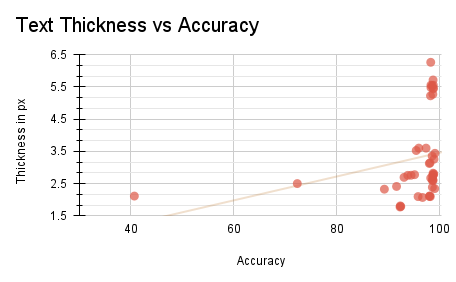
\includegraphics[width=\linewidth]{Figures/Figure_A.png}
    \caption{Text Thickness vs. Accuracy}
    \label{fig:FigA}
\end{figure}
\begin{figure}[h!]
    \centering
    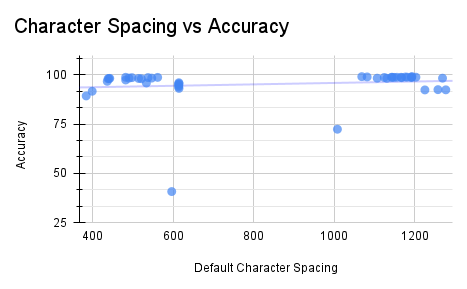
\includegraphics[width=\linewidth]{Figures/Figure_B.png}
    \caption{Character Spacing vs. Accuracy}
    \label{fig:FigB}
\end{figure}



This outcome revealed a limitation in the experimental design, as the selected fonts and their variations did not sufficiently challenge Tesseract’s character recognition capabilities. Consequently, this set of experiments was not successful in providing actionable insights. However, this failure was pivotal in refining the study's focus. It informed the design of the second series of testing, which employed a controlled baseline image to systematically evaluate Tesseract's performance under more variable conditions.

\subsection{Second Series of Testing}
The second series of tests yielded significantly more actionable results. Using the control image, I systematically evaluated Tesseract’s performance based on font size, letter spacing, and the number of characters in the image.

\begin{itemize}
\item \textbf{Font Size:} The experiments showed that the minimum font size required for Tesseract to detect text was 7 points, with the maximum size tested being 50 points. It is possible that larger font sizes could also work, but this was the upper limit tested in this experiment which can be seen in Figure~\ref{fig:FigC}. 
\begin{figure}[h!]
    \centering
    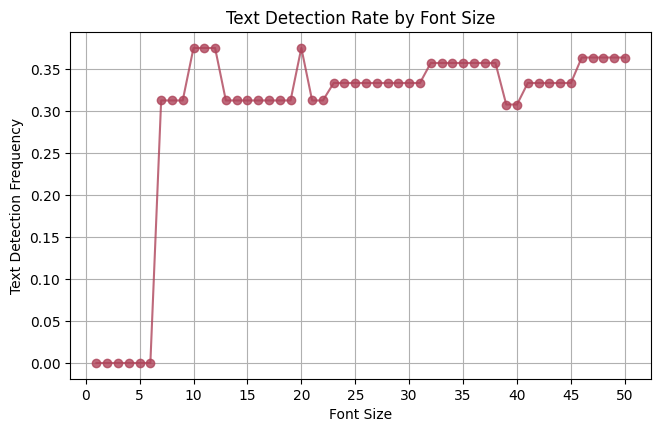
\includegraphics[width=\linewidth]{Figures/Figure_C.png}
    \caption{Text Detection Rate by Font Size}
    \label{fig:FigC}
\end{figure}
In a real-world context, the text in an image can be approximately 0.2 cm at its smallest and still be readable, provided the pixel density is sufficient to preserve the individual features of the character. This finding offers practical guidance on the smallest text sizes that Tesseract can reliably process.
\item \textbf{Letter Spacing:} The results revealed that an ideal letter spacing value is 1, as text detection decreased when spacing increased. Notably, a letter spacing value of 0 resulted in no text being detected. This outcome is likely because Tesseract’s character segmentation interpreted the grouped letters as a single unrecognizable character, failing to separate them for identification. Figure~\ref{fig:FigD} highlights these results. 
\begin{figure}[h!]
    \centering
    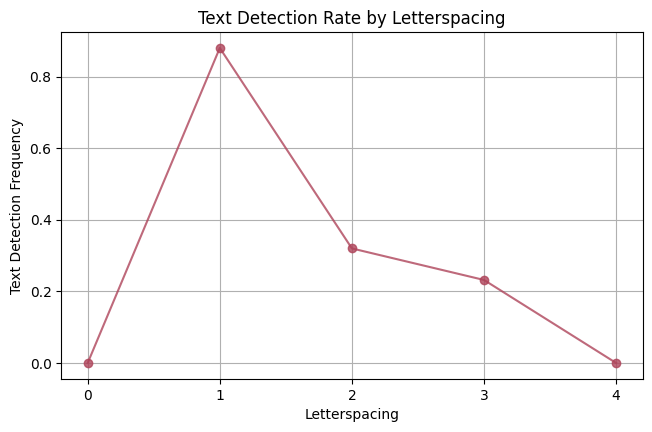
\includegraphics[width=\linewidth]{Figures/Figure_D.png}
    \caption{Text Detection Rate by Letter Spacing}
    \label{fig:FigD}
\end{figure}
For real-world applications, this means users should avoid excessive spacing between characters to ensure text detection. While this may not be an issue for standard printed or handwritten text, it could be particularly relevant for stylized designs, such as posters, where exaggerated spacing is used for aesthetic purposes. Future research should focus on testing incremental increases in spacing by single pixels to determine the exact threshold for text detection.
\item \textbf{Number of Letters:} Testing the number of letters in an image revealed a clear trend: text detection improved as the number of characters increased, as shown in Figure~\ref{fig:FigE}. 
\begin{figure}[h!]
    \centering
    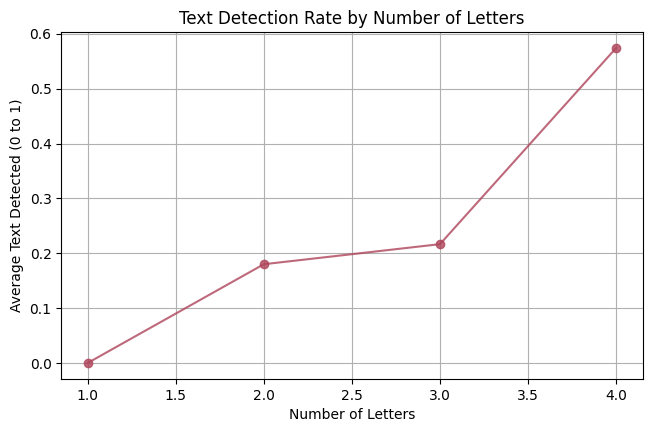
\includegraphics[width=\linewidth]{Figures/Figure_E.png}
    \caption{Text Detection Rate by Number of Letters}
    \label{fig:FigE}
\end{figure}
This result is unsurprising, as a higher number of characters provides more information for Tesseract to process. In a real-world context, this finding suggests that text segmentation strategies should ensure that each segment contains at least four characters to optimize detection and recognition. This aligns with common recommendations to break down text into manageable portions for OCR processing.
\item\textbf{Slant Value:} As shown in Figure~\ref{fig:FigF}, the ideal range for slant values lies between approximately -8 to 25 in the tested scale. Beyond this, slant values between -25 and 55 remain usable but exhibit progressively worse accuracy as they approach the extremes. Translating these values into real-world measurements, this corresponds to a slant range of roughly 50° to 150° for optimal accuracy and 30° to 160° for marginally usable results when measured from the base of the text. 
\begin{figure}[h!]
    \centering
    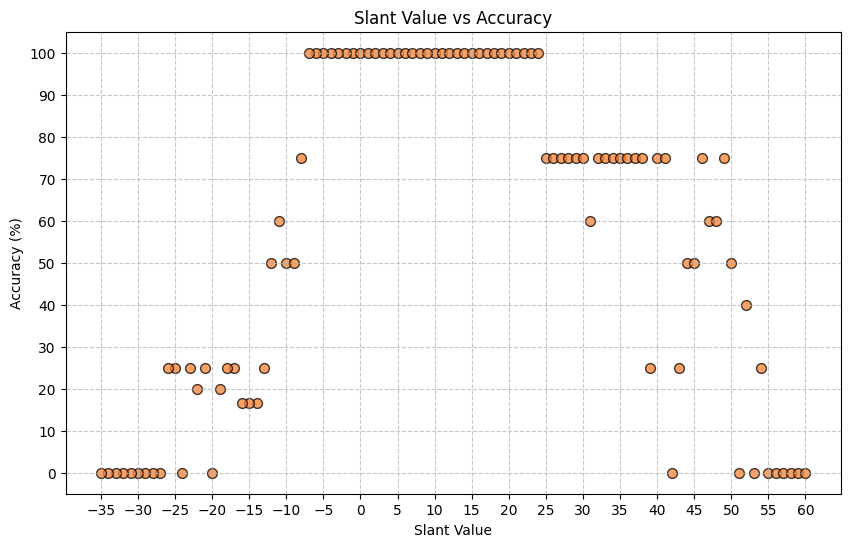
\includegraphics[width=\linewidth]{Figures/Figure_F.png}
    \caption{Slant Value vs Accuracy}
    \label{fig:FigF}
\end{figure}
This finding indicates that Tesseract is relatively good at dealing with slanted text such as what might occur in naturally skewed or imperfectly scanned documents. However, performance degrades significantly with more extreme slant angles. In practical terms, this suggests that preprocessing techniques to deskew images—such as affine transformations or angle corrections—should prioritize correcting slant to within the 50°–150° range to maximize recognition accuracy. For highly skewed text, automated angle detection and correction may be necessary to bring slant values into Tesseract’s optimal range. This also gives users the option to completely skip a deskewing step in their preprocessing if they know or are able to quickly calculate the slant of the the image they are scanning, potentially saving computation time especially when OCRing larger data sets.
\item \textbf{Salt and Pepper Noise:} Figure~\ref{fig:FigG} illustrates the impact of salt-and-pepper noise on Tesseract’s accuracy. At low noise levels (<10\%), accuracy remains near-perfect, with consistent text detection. However, accuracy begins to decline significantly as noise exceeds 20\%, and by 40\% noise strength, performance becomes highly unreliable. At noise levels above 60\%, Tesseract largely fails to detect text altogether. In real-world applications, this suggests that Tesseract is highly sensitive to noisy inputs, particularly at moderate-to-high noise levels. To mitigate this, preprocessing steps such as noise reduction techniques or image enhancement could significantly improve OCR outcomes. However, it also indicates that these steps can be skipped if the salt and pepper noise is low enough, saving both time and energy.
\begin{figure}[h!]
    \centering
    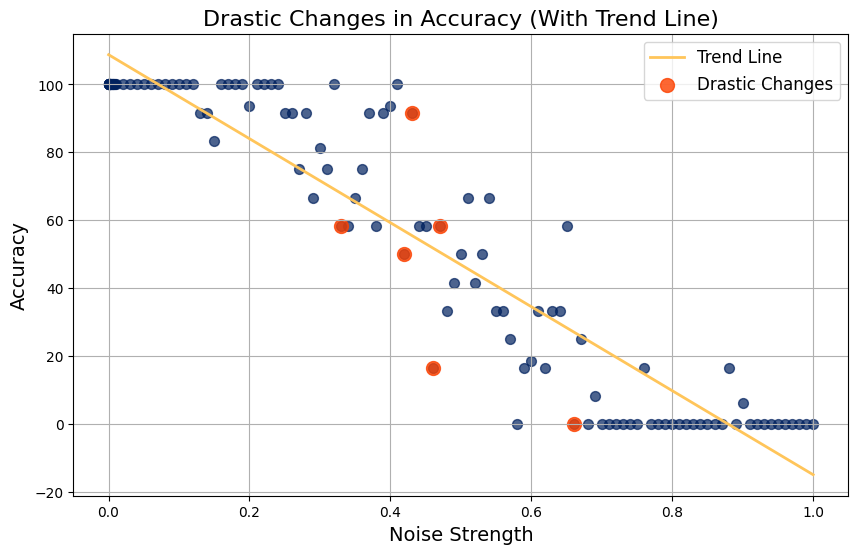
\includegraphics[width=\linewidth]{Figures/Figure_G.png}
    \caption{Salt and Pepper Percentage vs Accuracy}
    \label{fig:FigG}
\end{figure}
\item \textbf{White Space:} For white space, the experiments showed that the amount of white space required for text detection was heavily influenced by whether the space was only at the top or only at the bottom, as shown in Figure~\ref{fig:FigH}. When white space was evenly distributed above and below the text, Tesseract reliably detected text with a minimum of 5 pixels of space. However, when the white space was concentrated solely at the top or bottom, the minimum required increased to 9 pixels. This indicates that Tesseract's layout analysis struggles when text is offset within an image, requiring more buffer space in these cases. For practical applications, users should ensure that text is centered vertically within an image with sufficient white space on both sides to enhance detection. This finding is particularly relevant for processing images of documents or stylized layouts where uneven margins are common. Future studies could explore how multi-line text impacts these requirements or whether preprocessing can compensate for uneven white space distributions.
\begin{figure}[h!]
    \centering
    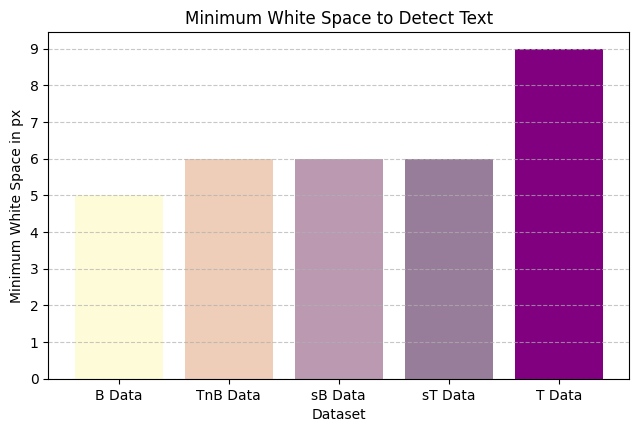
\includegraphics[width=\linewidth]{Figures/Figure_H.png}
    \caption{White Spacing Requirements}
    \label{fig:FigH}
\end{figure}
\item \textbf{Perlin Noise:}The results indicate that Tesseract can reliably detect text when Perlin noise strength is up to approximately 0.22. Beyond this threshold, the noise intensity causes Tesseract to fail completely. In numerical terms, this corresponds to the darkest shadow in the image being approximately 22\% darker than the background before the binarization process classifies it as black during the black-and-white conversion. For example, in Figure~\ref{fig:FigI}, the RGB value of the darkest shadow is 199 on a scale from 0 (black) to 255 (white). In a practical usage, shadows that are 20\% or less darker than the background (adding a small buffer) should not require preprocessing for lighting correction. However, if shadows are darker than 20\%, preprocessing steps, such as contrast enhancement or noise reduction, should be applied to ensure reliable OCR performance.
These findings can help users determine if their images or datasets require preprocessing for lighting issues and hopefully help reduce computational and user time. 
\end{itemize}
\begin{figure}[h!]
    \centering
    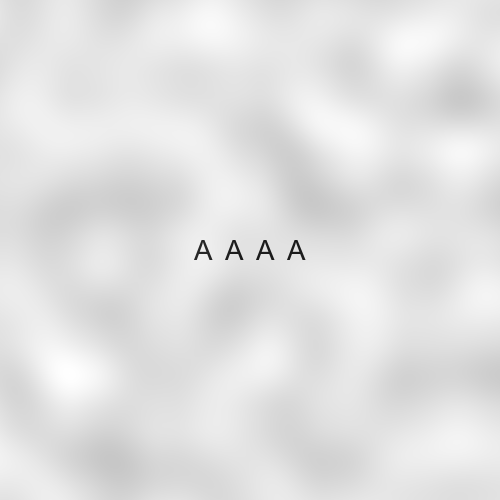
\includegraphics[width=\linewidth]{Figures/Figure_I.png}
    \caption{.219 Perlin Noise Strenght Image}
    \label{fig:FigI}
\end{figure}
The results of this study provide actionable insights into Tesseract's performance under various conditions, highlighting both its strengths and limitations. While the first series of tests with diverse fonts revealed little variability in accuracy, the second series offered meaningful findings by systematically evaluating specific parameters. Key takeaways include Tesseract's ability to handle small font sizes, the critical importance of balanced white space, and its sensitivity to slant angles and noise levels. Practical recommendations, such as skipping preprocessing steps under specific conditions (e.g., low noise or minimal shadow contrast), can help users optimize OCR workflows. These findings not only enhance our understanding of Tesseract's operational boundaries but also provide a framework for efficient preprocessing strategies that can save computational resources and time, particularly for large datasets. Future work should explore how these parameters interact in more complex scenarios, such as handwritten text or multi-layered distortions, to further refine the tool’s usability.


\section{Ethical Considerations}
Although this project does not create a tool, it is still important to consider the ethics of creating and using computer vision tools like Tesseract. For Tesseract, there are two main ethical considerations for this project and others similar to it: consent to have people’s data/Intellectual-Property fed to the dataset and consent to use the Tesseract on another person’s work. 
\subsection{Consent in Dataset Inclusion}
Machine learning models like Tesseract rely on extensive datasets for training. However, it is unclear if these datasets were created with the informed consent of the creators of the included resources. The data gathered from the resources may include copyrighted or private information, which raises concerns about potential breaches of intellectual property and personal rights. It is possible that some consent was obtained, but it may not have been informed consent. For example, individuals could unknowingly agree to data usage through opaque mechanisms such as website cookies or dense legal language. This lack of clarity underscores the need for stricter standards for dataset composition and the ethical collection of training resources.
\subsection{Responsible use of OCR Technology}
The advancement of OCR technology, while easing mundane work like data entry, also facilitates the unauthorized extraction and spreading of sensitive or protected information. For example, individuals may use OCR to scan and replicate copyrighted material, such as books or scientific papers, without obtaining proper permissions. While this capability can promote accessibility and knowledge sharing in positive ways, it also poses risks to the financial viability of publishers, researchers, and independent creators who rely on revenue from their work. Such practices could result in reduced funding for future research and discourage the production of creative works, particularly by individuals or small organizations operating on narrow profit margins. Beyond intellectual property concerns, OCR technology could also be used to breach  personal privacy. A bad actor might use OCR to extract sensitive data from medical documents, personal identification records, or other private materials via images photographed in-person or via a compromised web cam.  These type breaches could have severe consequences such as identity theft and blackmail. On the more extreme end, a malicious person may exploit medical information to directly harm a person by exploiting an allergy or other health issues.

\paragraph{} These risks highlight the dual responsibility of developers and users to ensure OCR tools are applied ethically, with safeguards against misuse. Given the growing reliance on OCR technologies like Tesseract, it is essential that their development and application align with ethical principles emphasizing transparency, informed consent, and respect for privacy and intellectual property. Proactively addressing these concerns is critical to building trust and ensuring the responsible and equitable use of such technologies.

\section{Appendices}
\subsection{Replication Instructions}

To replicate this project, ensure you have the following tools and configurations set up. All instructions are designed to be future-proof by specifying exact versions for software and packages used.

\begin{itemize}
    \item \textbf{Operating System:} Windows 10 or Windows 11.
    \item \textbf{Code Editor:} Visual Studio Code (v1.96.0), with the Git Graph extension for version control.
    \item \textbf{Version Control:} GitHub Desktop.
    \item \textbf{Python Environment:}
    \begin{itemize}
        \item Python 3.13.0
        \item \textbf{Python Libraries:}
        \begin{itemize}
            \item fonttools 4.54.1
            \item matplotlib 3.9.2
            \item numpy 2.1.2
            \item opencv-python 4.10.0.84
            \item packaging 24.1
            \item pandas 2.2.3
            \item pillow 11.0.0
            \item pip 24.3.1
            \item pycparser 2.22
            \item pyparsing 3.2.0
            \item pytesseract 0.3.13
            \item setuptools 75.3.0
            \item six 1.16.0
            \item svgwrite 1.4.3
            \item tesseract 0.1.3
            \item tinycss2 1.4.0
            \item tzdata 2024.2
            \item webencodings 0.5.1
        \end{itemize}
    \end{itemize}
    \item \textbf{Tesseract OCR:} Version 5.4.0.20240606
    \item \textbf{Leptonica:} Version 1.84.1
\end{itemize}

\textbf{Setup Instructions:}
\begin{enumerate}
    \item Install Python 3.13.0 from the official Python website and ensure pip is updated to version 24.3.1 using the command:
    \texttt{python -m pip install --upgrade pip}.
    \item Install the required Python libraries using:
\begin{verbatim}
pip install fonttools==4.54.1 \
    matplotlib==3.9.2 \
    numpy==2.1.2 \
    opencv-python==4.10.0.84 \
    packaging==24.1 \
    pandas==2.2.3 \
    pillow==11.0.0 \
    pycparser==2.22 \
    pyparsing==3.2.0 \
    pytesseract==0.3.13 \
    setuptools==75.3.0 \
    six==1.16.0 \
    svgwrite==1.4.3 \
    tesseract==0.1.3 \
    tinycss2==1.4.0 \
    tzdata==2024.2 \
    webencodings==0.5.1
\end{verbatim}
    \item Install Tesseract OCR v5.4.0.20240606 and Leptonica 1.84.1 from their respective official sources. Ensure Tesseract is accessible via the system path by verifying it with the command:
    \texttt{tesseract -v}.
    \item Set up version control using GitHub Desktop and initialize your repository. Use the Git Graph extension in Visual Studio Code for visualization.
\end{enumerate}
\subsection{Code Architecture Overview}

The code for this project is structured under a main directory called \texttt{Pytesseract\_analysis}, organized to facilitate debugging, extension, and ease of understanding. Within this directory, several subfolders serve specific purposes based on the development stages and functionality.

The main folder includes auto-generated directories such as \texttt{.vscode} and \_\_pycache\_\_. These folders are automatically created by the Visual Studio Code environment and Python, respectively, and are not intended for modification. Their primary purpose is to maintain editor settings and optimize runtime performance.

Within the directory, the \texttt{Code\_Experiments} folder houses files developed during the early phases of experimentation. While not directly relevant to the final implementation, this folder contains useful code snippets and concepts from failed or preliminary tests that could inspire future development.

The \texttt{Image Processing} folder is another auxiliary directory, created as part of an attempt to implement preprocessing techniques identified during the research phase. Although these techniques were not incorporated into the final project, the folder remains a valuable resource for developers who wish to extend the project by integrating additional preprocessing methods.

The first and second series of experiments are managed within dedicated folders named \texttt{First Series of Experiments} and \texttt{Second Series of Experiments}. The \texttt{First Series of Experiments} folder contains the code used to generate the dataset of font images, including subfolders for fonts and images. These subfolders are organized by experiment type and include the text input used during testing, such as the quote from "Frankenstein." This structure makes it easy to reproduce or modify the dataset generation process for further analysis.

The \texttt{Second Series of Experiments} folder is more streamlined, containing the code and data used to test specific parameters in controlled conditions. This includes the control image and scripts that run Tesseract’s analysis on generated test cases. The organization within this folder is parameter-based, enabling clear identification of the specific experiments performed and simplifying potential extensions or modifications to the parameter testing process.

Finally, the \texttt{Research Documents} folder contains various references and supporting materials that informed the development of the project. Although not directly related to the code, these documents provide valuable context and serve as a resource for understanding the decisions made during the research phase.

\printbibliography

\end{document}
